\begin{figure*}[tbp]
  \centering
  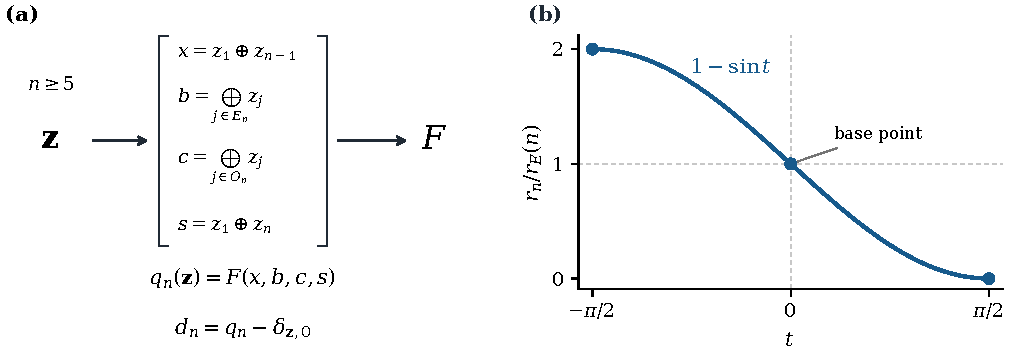
\includegraphics[width=\textwidth]{figures/fig1_unified.pdf}
  \caption{覆盖全部 $n\geq5$ 的统一相位变形。
  (a) 四个线性 Boolean 特征输入同一个核 $F$；从支持中删去的唯一点是物理全零串 $\mathbf z=0$。内部奇偶块 $E$、$O$ 的定义见正文。
  (b) 区间 $[-\pi/2,\pi/2]$ 上的归一化共同 Bloch 半径 $1-\sin t$。
  三个标记点依次为增强端点、$t=0$ 处的指定 EJM，以及所有单比特边缘均完全混合的端点。 绘图代码由 OpenAI Codex（GPT-6）辅助编写，并按文中公式核对。}
  \label{fig:unified}
\end{figure*}
